\section{Background and Related Work}

\begin{figure}[t]
    \vspace{-5pt}
    \centering
    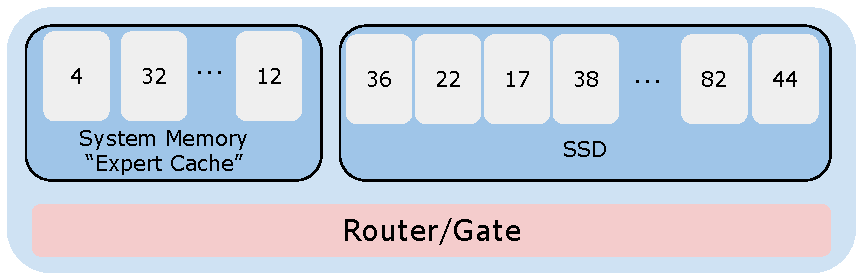
\includegraphics[width=\columnwidth]{figures/expert_storage_cropped.pdf}
    \vspace{-10pt}
    \caption{Selected experts may reside in memory or SSD}
    \label{fig:transformer_vs_moe}
    \vspace{-5pt}
\end{figure}

\subsection{Hardware Architecture and Constraints}
Modern edge AI platforms, \cite{amd-2025-ryzen-ai-9-hx-370,feng2025profilingapplesiliconperformance,snapdragonX,LunarLake}, employ a Unified Memory Architecture (UMA) in which the CPU, integrated GPU (iGPU), and other compute units share a common physical memory pool. Unlike discrete GPU systems, where host-to-device transfers often dominate MoE inference latency \cite{xue2025moeinfinityefficientmoeinference,gavhane2025moebeyondlearningbasedexpertactivation,song2025promoefastmoebasedllm}, UMA eliminates explicit host-to-device transfers in most cases through shared memory. However, when MoE models exceed available memory capacity and inactive experts are offloaded to an SSD, decode throughput becomes bottlenecked by expert loading latency from SSD  \cite{kim2026flashmoereducingssdio}.

\subsection{SSD-Backed MoE Inference}
MoE architectures \cite{shazeer2017outrageouslylargeneuralnetworks,zhang2022moeficationtransformerfeedforwardlayers,fedus2022switchtransformersscalingtrillion} trade the single dense feed-forward network (FFN) found in classical transformer models \cite{vaswani2017attention} for many router-selected, smaller FFNs (experts). Although sparse activation primarily reduces per-token computation, it also allows inactive experts to be offloaded to secondary storage, making deployment of large MoE models feasible on memory-constrained systems. Recent work has studied SSD-backed inference to explore this opportunity. For example, FlashMoE \cite{kim2026flashmoereducingssdio} directly addresses the SSD I/O bottleneck by employing ML-based cache replacement policies to keep the most relevant experts resident in memory. While somewhat effective, this is a reactive cache policy optimization; in contrast, ExpertAhead performs proactive, asynchronous SSD prefetches, allowing the system to actively hide load latency on top of implementing an expert cache management policy.

\subsection{Expert Prediction and Prefetching}
Expert prefetching is a widely studied technique for accelerating MoE inference, most commonly deployed to move experts from host CPU memory into discrete GPU memory \cite{xue2025moeinfinityefficientmoeinference,gavhane2025moebeyondlearningbasedexpertactivation,song2025promoefastmoebasedllm,zhu2025preattentionexpertpredictionprefetching, zhang2025daopdataawareoffloadingpredictive}. 

Existing prefetching approaches can be classified by their prediction horizon. \textbf{Short-horizon methods} operate intralayer: predicting expert usage within the same layer for the current token \cite{zhu2025preattentionexpertpredictionprefetching}, or interlayer: predicting activations in future layers. Interlayer prediction has been studied by applying a future layer's gating function directly to current hidden states \cite{eliseev2023fastinferencemixtureofexpertslanguage, zhu2026daliworkloadawareoffloadingframework, fang2025fatefastedgeinference, yao2024exploitinginterlayerexpertaffinity}, utilizing offline-trained predictors \cite{song2025promoefastmoebasedllm, zhang2026duoservemoedualphaseexpertprefetch, yi2025edgemoeempoweringsparselarge, gavhane2025moebeyondlearningbasedexpertactivation}, or leveraging an Expert Activation Matrix (EAM) \cite{xue2025moeinfinityefficientmoeinference}. Conversely, \textbf{long-horizon methods} extend the prediction window across multiple future tokens, typically by leveraging speculative decoding \cite{wang2025moespeqspeculativequantizeddecoding, chen2025spmoespeculativedecodingprefetching} to predict tokens and expert activations. However, the memory overhead required to maintain a secondary draft model makes this approach poorly suited for memory-constrained edge deployments. Allocating memory for this draft model reduces memory available for caching experts, which increases SSD accesses, the fundamental bottleneck, potentially offsetting the latency benefits of speculative decoding.

% For example, storing a draft model of the same relative size as used in \cite{chen2025spmoespeculativedecodingprefetching} would yield a 41\% decode slowdown compared to an equal-memory expansion of the expert cache in our system.

ExpertAhead occupies a practical middle ground: we utilize a lightweight predictor model to forecast expert usage for the next $S$ tokens. This multi-token horizon provides significantly more time to hide SSD loading latency than short-horizon methods, while avoiding the memory overhead of speculative draft models.

\subsection{Modified Expert Activation}
Beyond prefetching, reducing the volume of required expert loads is critical. Current approaches achieve this by pruning or dropping unimportant experts \cite{chen2022taskspecificexpertpruningsparse, qiu2025demonsdetailimplementingload} or by dynamically substituting router-selected SSD-resident experts to avoid disk reads \cite{skliar2025mixturecacheconditionalexpertsefficient, zhu2026smoealgorithmsystemcodesignpushing}. However, relying solely on cache-aware routing inherently limits model quality by not using all of the router-selected experts. Inspired by the evaluation framework in SpecMD \cite{hoang2026specmdcomprehensivestudyspeculative}, which assesses the combination of predictive and reactive techniques, ExpertAhead-CC implements predictive prefetching with cache-conditional routing. This ensures the system only substitutes an expert when it is not predicted or prefetched in time, thereby maximizing throughput while minimizing perplexity degradation.